Gpredict is an open source program to track satellites and predict their respective orbits. 
\newline
In general a satellite tracking program predicts the flight data of a satellite, like the position and velocity, by calculating values given by recieved Keplerian Elements, describing the orbit, using the \textit{\acs{NORAD} SGP4/SDP4} algorithm \cite{hoots_spacetrack_1980}. After these values are retrieved other values like the bearing, distance and visibility can be calculated with the calculated orbit data and known location of the \acp{GCC} for a certain date and time. A general overview how a satellite tracking system works can be seen at \ref{SatTrackOverview}. \cite{csete_gpredict_2011}
\newline
\begin{figure}[ht!]
\centering
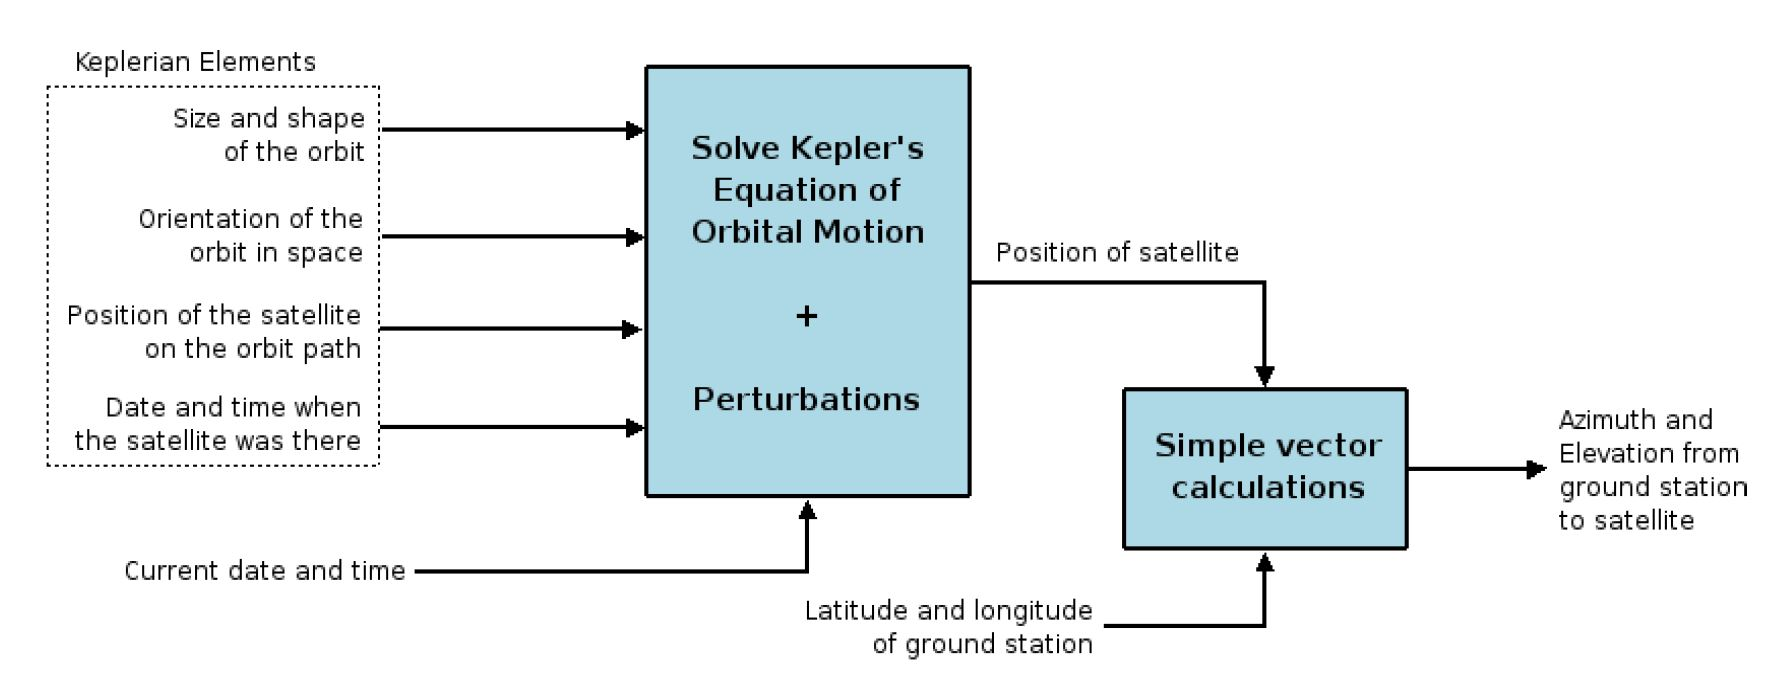
\includegraphics[width=120mm]{PICs/functional_overview_satellite_tracking_prog.jpg}
\caption[Functionality of a satellite tracking program - licensed under the \acl{GNU GPL} \cite{csete_gpredict_2011}]{Functionality of a satellite tracking program - licensed under the \acl{GNU GPL} \label{SatTrackOverview}}
\end{figure}